\chapter*{گزارش فنی پروژه نویز خوانش چهار کیوبیتی}

\section{هدف و تصویر کلی}

هدف این گزارش، مستندسازی یک پایپلاین کامل برای مدل‌سازی نویز خوانش در یک سامانه چهار کیوبیتی است. پروژه از داده‌های خام تجربی \lr{IQ} شروع می‌شود، از روی آن‌ها ماتریس‌های خطای خوانش را استخراج می‌کند، سپس این نویزها را روی مدارهای کوانتومی اعمال می‌کند و در نهایت با یک مدل یادگیری ماشین تلاش می‌کند توزیع احتمال نویزی را به توزیع ایده‌آل بازگرداند.

دو فایل اصلی پروژه چنین نقشی دارند:
\begin{itemize}
	\item \lr{readout\_matrix.ipynb}: بارگذاری داده‌های تجربی، آموزش تفکیک‌کننده \lr{IQ}، استخراج ماتریس‌های $2\times2$ و $16\times16$؛
	\item \lr{noisy\_4q\_zzfeaturemap.ipynb}: ساخت مدار، اعمال سه نوع نویز، تولید دیتاست، آموزش \lr{MLP} و ارزیابی با \lr{fidelity}.
\end{itemize}

در کل پروژه یک قرارداد مهم حفظ می‌شود: ماتریس نویز خوانش به صورت
\begin{equation}
	A_{ij}=P(\text{measured}=j \mid \text{prepared}=i)
	\label{eq:assignment-convention}
\end{equation}
تعریف شده است. بنابراین سطرها حالت آماده‌سازی و ستون‌ها حالت اندازه‌گیری هستند و هر سطر جمع یک دارد. این همان قرارداد مورد استفاده در \lr{Qiskit ReadoutError} است.

\section{معماری کلی خط لوله پروژه}

پروژه یک مسیر پیوسته از داده خام تا ارزیابی mitigation دارد. شکل~\ref{fig:pipeline} این مسیر را به صورت یک سیستم واحد نشان می‌دهد؛ نه چند آزمایش جدا.

\begin{figure}[htbp]
\centering
\resizebox{0.95\textwidth}{!}{%
\begin{tikzpicture}[
	node distance=8mm and 10mm,
	box/.style={draw, rounded corners, align=center, minimum width=3.2cm, minimum height=1.0cm, fill=blue!6},
	small/.style={draw, rounded corners, align=center, minimum width=2.8cm, minimum height=0.9cm, fill=orange!8},
	metric/.style={draw, rounded corners, align=center, minimum width=2.6cm, minimum height=0.9cm, fill=green!8},
	arrow/.style={-{Stealth[length=2.2mm]}, thick}
]
\node[box] (iq) {داده تجربی \lr{IQ}\\ \lr{16} حالت $\times$ \lr{1000} shot};
\node[box, below=of iq] (lda) {طبقه‌بندی \lr{IQ}\\ \lr{LDA}};
\node[box, below=of lda] (a2) {ماتریس‌های $2\times2$\\ تک‌کیوبیتی};
\node[box, below=of a2] (a16) {ماتریس همبسته\\ $16\times16$};
\node[box, right=18mm of a16] (sim) {شبیه‌سازی مدار\\ \lr{Qiskit Aer}};
\node[small, above=of sim] (ideal) {$\mathbf{p}_{\mathrm{ideal}}$};
\node[small, below=of sim] (noisy) {$\mathbf{p}_{\mathrm{noisy}}$};
\node[box, right=18mm of sim] (mlp) {مدل \lr{MLP}\\ mitigation};
\node[small, right=18mm of mlp] (out) {$\hat{\mathbf{p}}_{\mathrm{ideal}}$};
\node[metric, below=14mm of out] (eval) {Fidelity / KL / L1};

\draw[arrow] (iq) -- (lda);
\draw[arrow] (lda) -- (a2);
\draw[arrow] (a2) -- (a16);
\draw[arrow] (a16.east) -- ++(6mm,0) |- (sim.west);
\draw[arrow] (sim) -- (ideal);
\draw[arrow] (sim) -- (noisy);
\draw[arrow] (ideal.east) -| (mlp.north);
\draw[arrow] (noisy.east) -- (mlp.west);
\draw[arrow] (mlp) -- (out);
\draw[arrow] (out) -- (eval);
\end{tikzpicture}%
}
\caption{معماری کلی خط لوله: از داده \lr{IQ} تا استخراج ماتریس نویز، تولید توزیع ایده‌آل/نویزی، mitigation با \lr{MLP} و ارزیابی.}
\label{fig:pipeline}
\end{figure}

\textbf{دو شاخه اصلی:}
\begin{enumerate}
	\item \textbf{شاخه کالیبراسیون:} داده \lr{IQ} $\rightarrow$ \lr{LDA} $\rightarrow$ ماتریس‌های نویز؛
	\item \textbf{شاخه mitigation:} مدار کوانتومی $\rightarrow$ $\mathbf{p}_{\mathrm{ideal}}$ و $\mathbf{p}_{\mathrm{noisy}}$ $\rightarrow$ \lr{MLP} $\rightarrow$ $\hat{\mathbf{p}}_{\mathrm{ideal}}$.
\end{enumerate}
شاخه اول «مدل نویز سخت‌افزار» را می‌سازد؛ شاخه دوم از آن برای تولید دیتاست و ارزیابی استفاده می‌کند.

\section{داده‌های تجربی \lr{IQ}}

\subsection{ساختار فایل‌ها}

داده‌های تجربی در پوشه \lr{quadrature\_data\_4qubits} قرار دارند. برای هر یک از ۱۶ حالت پایه محاسباتی یک فایل وجود دارد؛ از \lr{0000.txt} تا \lr{1111.txt}.
هر فایل چهار خط دارد؛ هر خط مربوط به یک کیوبیت است و شامل ۱۰۰۰ نمونه مختلط از نوع
\[
	z = I+iQ
\]
است. بنابراین برای هر حالت آماده‌سازی، ۱۰۰۰ shot و برای کل پروژه
\[
	16 \times 1000 = 16000
\]
نمونه چهارکیوبیتی داریم. پس از بارگذاری:
\[
	X \in \mathbb{C}^{16000\times4}, \qquad
	Y \in \{0,1\}^{16000\times4}.
\]
در این نمایش، $X[n,q]$ نمونه \lr{IQ} کیوبیت $q$ در shot شماره $n$ و $Y[n,q]$ بیت آماده‌سازی همان کیوبیت است.

\subsection{برچسب‌گذاری و ترتیب بیت‌ها}

برچسب‌ها از نام فایل به دست می‌آیند. در کد، تابع \lr{bits\_from\_filename} نام فایل را خوانده و برای سازگاری با ترتیب داخلی پروژه، بیت‌ها را معکوس می‌کند. قرارداد اندیس‌گذاری حالت‌ها چنین است:
\begin{equation}
	i=b_1+2b_2+4b_3+8b_4.
	\label{eq:bits-to-int}
\end{equation}
پس $b_1$ کم‌ارزش‌ترین بیت است و $b_4$ پرارزش‌ترین بیت. این قرارداد باید در همه بخش‌ها، از ساخت ماتریس نویز تا تبدیل شمارش‌های \lr{Qiskit} به بردار احتمال، یکسان بماند.

\subsection{ابرهای \lr{IQ} و معنای فیزیکی آن‌ها}

در اندازه‌گیری dispersive، خروجی هر shot یک نقطه در صفحه \lr{IQ} است. اگر کیوبیت در حالت $|0\rangle$ آماده شده باشد، نقاط باید اطراف یک ابر و اگر در $|1\rangle$ آماده شده باشد اطراف ابر دیگری قرار گیرند. هرچه این دو ابر جدا‌تر باشند، readout fidelity بالاتر است. همپوشانی ابرها همان ناحیه‌ای است که در آن تفکیک‌کننده ممکن است $0$ را $1$ یا $1$ را $0$ تشخیص دهد.

\begin{figure}[htbp]
\centering

\includegraphics[width=\textwidth]{clouds.png}
\caption{ابرهای \lr{IQ} برای دو حالت چهارکیوبیتی \lr{0101} و \lr{1010}. هر پنل مربوط به یک کیوبیت است. جدایی و همپوشانی ابرها نشان می‌دهد خطای خوانش برای هر کیوبیت چقدر است و آیا crosstalk بین کیوبیت‌ها وجود دارد یا نه.}
\label{fig:iq-clouds}
\end{figure}

شکل~\ref{fig:iq-clouds} چند نکته مهم را نشان می‌دهد. نخست، جدایی ابرها برای همه کیوبیت‌ها یکسان نیست، پس ماتریس‌های تک‌کیوبیتی نباید الزاماً مشابه باشند. دوم، شکل ابرها فقط تابع بیت همان کیوبیت نیست و حالت کلی چهارکیوبیتی هم می‌تواند مرکز یا پراکندگی ابر را تغییر دهد. این رفتار نشانه‌ای از \lr{crosstalk} و دلیل اصلی نیاز به ماتریس همبسته $16\times16$ است.

\section{استخراج ماتریس‌های نویز خوانش}

\subsection{مدل \lr{Linear Discriminant Analysis}}

در بخش اول پروژه، برای هر کیوبیت یک مدل \lr{LinearDiscriminantAnalysis} یا \lr{LDA} آموزش داده شده است. ورودی مدل برای کیوبیت $q$ بردار دوبعدی
\[
	\mathbf{x}=(I,Q)^\top
\]
و برچسب آن $0$ یا $1$ است. داده‌ها با \lr{train\_test\_split} و نسبت $80/20$ تقسیم می‌شوند و ویژگی‌ها قبل از آموزش با \lr{StandardScaler} نرمال‌سازی می‌شوند.

\lr{LDA} فرض می‌کند دو کلاس $0$ و $1$ در صفحه \lr{IQ} تقریباً توزیع گاوسی با کواریانس مشترک دارند. برای کلاس $k$ تابع امتیاز به صورت
\begin{equation}
	\delta_k(\mathbf{x}) =
	\mathbf{x}^{\top}\Sigma^{-1}\mu_k
	-\frac{1}{2}\mu_k^{\top}\Sigma^{-1}\mu_k
	+\log \pi_k
	\label{eq:lda-score}
\end{equation}
نوشته می‌شود. در این رابطه $\mu_k$ میانگین کلاس، $\Sigma$ کواریانس مشترک و $\pi_k$ prior کلاس است. مدل نمونه را به کلاسی نسبت می‌دهد که $\delta_k$ بزرگ‌تری دارد. برای دو کلاس، مرز تصمیم یک خط در صفحه \lr{IQ} است:
\[
	\mathbf{w}^{\top}\mathbf{x}+w_0=0,\qquad
	\mathbf{w}=\Sigma^{-1}(\mu_1-\mu_0).
\]

انتخاب \lr{LDA} برای این پروژه منطقی است، چون مسئله تفکیک \lr{IQ} دوبعدی است، مدل پایدار و قابل تفسیر است و هدف اصلی صرفاً بیشینه کردن accuracy نیست؛ هدف ساختن تخمینی پایدار از احتمال‌های $P(m|p)$ است. در نوت‌بوک، \lr{QDA} نیز آزمایش شده است، اما \lr{LDA} به عنوان گزینه ساده‌تر و پایدارتر انتخاب شده است.

\subsection{ماتریس‌های تک‌کیوبیتی $2\times2$}

پس از آموزش مدل کیوبیت $q$، خروجی model روی داده test با برچسب واقعی مقایسه می‌شود. ماتریس تخصیص تک‌کیوبیتی از ماتریس confusion نرمال‌شده ساخته می‌شود:
\begin{equation}
	A^{(q)}=
	\begin{pmatrix}
	P(m_q=0|p_q=0) & P(m_q=1|p_q=0)\\
	P(m_q=0|p_q=1) & P(m_q=1|p_q=1)
	\end{pmatrix}.
	\label{eq:single-assignment}
\end{equation}
در این ماتریس، عناصر قطری fidelity خوانش حالت‌های $0$ و $1$ هستند و عناصر غیرقطری احتمال خطای flip در خوانش را نشان می‌دهند. برای مثال، در یکی از اجراها ماتریس کیوبیت ۱ تقریباً چنین بوده است:
\[
	A^{(1)}\approx
	\begin{pmatrix}
	0.794 & 0.206\\
	0.369 & 0.631
	\end{pmatrix}.
\]
این یعنی وقتی کیوبیت ۱ در $|0\rangle$ آماده شده، حدود $20.6\%$ احتمال دارد $1$ خوانده شود، و وقتی در $|1\rangle$ آماده شده، حدود $36.9\%$ احتمال دارد $0$ خوانده شود.

\subsection{ماتریس همبسته $16\times16$}

برای ساخت ماتریس کامل، چهار مدل تک‌کیوبیتی روی کل دیتاست اعمال می‌شوند و برای هر shot یک بیت‌رشته پیش‌بینی‌شده $\hat{\mathbf{b}}$ به دست می‌آید. سپس برای هر حالت آماده‌سازی $i$ و حالت اندازه‌گیری $j$ شمارش انجام می‌شود:
\begin{equation}
	M_{ij}
	=
	\frac{1}{N_i}
	\sum_{n:\,Y_n=\mathrm{bits}(i)}
	\mathbb{1}\left[
	\mathrm{bits\_to\_int}(\hat{\mathbf{b}}_n)=j
	\right].
	\label{eq:full-matrix}
\end{equation}
این ماتریس همان کانال کلاسیک خوانش چهارکیوبیتی است:
\[
	\mathbf{p}_{\mathrm{measured}}
	=
	\mathbf{p}_{\mathrm{prepared}}\,M.
\]
اعتبارسنجی اصلی این است که برای هر سطر
\[
	\sum_{j=0}^{15} M_{ij}=1.
\]
در اجرای موجود، میانگین عناصر قطری این ماتریس حدود
\[
	\bar{F}_{\mathrm{diag}}=\frac{1}{16}\sum_i M_{ii}\approx0.385
\]
بوده است. این عدد نشان می‌دهد خوانش چهارکیوبیتی دقیقاً به همان حالت آماده‌شده، به دلیل ضرب خطاهای چند کیوبیت و همبستگی‌ها، fidelity نسبتاً پایینی دارد.

\subsection{اعتبارسنجی ماتریس‌های نویز}

استخراج ماتریس کافی نیست؛ باید مطمئن شویم خروجی یک \emph{کانال احتمال معتبر} است. در غیر این صورت نمی‌توان آن را در شبیه‌سازی یا mitigation استفاده کرد.

\textbf{بررسی‌های اصلی:}
\begin{align}
	A_{ij} &\ge 0 && \text{(غیرمنفی بودن)} \label{eq:val-nonneg}\\
	\sum_{j} A_{ij} &= 1 && \text{(نرمال‌سازی سطری)} \label{eq:val-row}\\
	\bar{A}_{ii} &= \frac{1}{16}\sum_i A_{ii} && \text{(رفتار قطری)} \label{eq:val-diag}\\
	M &\neq A^{(1)}\otimes A^{(2)}\otimes A^{(3)}\otimes A^{(4)} && \text{(عدم استقلال)} \label{eq:val-kron}
\end{align}

\begin{table}[htbp]
\centering
\caption{چک‌لیست اعتبارسنجی ماتریس نویز}
\label{tab:matrix-validation}
\begin{tabular}{lll}
\toprule
بررسی & شرط & معنی فیزیکی \\
\midrule
غیرمنفی & $A_{ij}\ge0$ & احتمال منفی معنا ندارد \\
نرمال‌سازی & $\sum_j A_{ij}=1$ & هر حالت آماده به توزیع کامل می‌رود \\
قطری & $\bar{A}_{ii}\approx0.39$ & میانگین fidelity خوانش \\
مقایسه & $M\neq M_{\mathrm{indep}}$ & وجود crosstalk / correlation \\
\bottomrule
\end{tabular}
\end{table}

این اعتبارسنجی تضمین می‌کند ماتریس استخراج‌شده را می‌توان مستقیماً به عنوان کانال readout در تولید $\mathbf{p}_{\mathrm{noisy}}$ استفاده کرد. اگر قرارداد سطری \lr{Qiskit} رعایت نشود یا ordering بیت‌ها جابه‌جا شود، ماتریس از نظر ریاضی stochastic به نظر می‌رسد اما فیزیکاً اشتباه خواهد بود.

\subsection{چرا ماتریس $16\times16$ برابر کرونکر چهار ماتریس $2\times2$ نیست؟}

اگر خطای خوانش چهار کیوبیت کاملاً مستقل بود، ماتریس کامل از کرونکر محصول ماتریس‌های تک‌کیوبیتی به دست می‌آمد:
\begin{equation}
	M_{\mathrm{indep}}
	=
	A^{(4)}\otimes A^{(3)}\otimes A^{(2)}\otimes A^{(1)}.
	\label{eq:kron}
\end{equation}
اما این فقط تحت فرض استقلال معتبر است. در داده تجربی، ابرهای \lr{IQ} نشان می‌دهند حالت دیگر کیوبیت‌ها می‌تواند توزیع خوانش یک کیوبیت را جابه‌جا کند. بنابراین
\[
	M \neq M_{\mathrm{indep}}
\]
و همین اختلاف حامل اطلاعات فیزیکی مهم درباره crosstalk، خطاهای همبسته و غیرقابل فاکتورسازی بودن خوانش است.

به بیان دیگر، ماتریس‌های $2\times2$ پاسخ متوسط هر کیوبیت را جداگانه خلاصه می‌کنند، اما ماتریس $16\times16$ پاسخ کل register را به صورت مشترک ثبت می‌کند. انتظار برابری این دو فقط در یک مدل ایده‌آل مستقل درست است، نه در سخت‌افزار واقعی.

\section{مدارهای کوانتومی استفاده‌شده در بخش دوم}

در بخش دوم، از دو خانواده مدار برای تولید توزیع احتمال ایده‌آل و نویزی استفاده شده است. در هر نمونه، بردار پارامتر
\[
	\boldsymbol{\theta}=(\theta_1,\theta_2,\theta_3,\theta_4)
\]
به طور تصادفی از بازه $[0,\pi]^4$ انتخاب می‌شود.

\subsection{مدار مستقل \lr{Independent RY}}

\begin{figure}[htbp]
\centering

\includegraphics[width=0.7\textwidth]{independent_circuit.png}
\caption{مدار مستقل شامل چهار گیت $R_y(\theta_i)$ و اندازه‌گیری نهایی. این مدار درهم‌تنیدگی ایجاد نمی‌کند و توزیع خروجی آن فاکتورسازی‌شده است.}
\label{fig:independent-circuit}
\end{figure}

در این مدار روی هر کیوبیت فقط یک گیت $R_y$ اعمال می‌شود:
\begin{equation}
	R_y(\theta)=e^{-i\theta Y/2}.
\end{equation}
اثر آن روی حالت اولیه $|0\rangle$ چنین است:
\begin{equation}
	R_y(\theta)|0\rangle
	=
	\cos\frac{\theta}{2}|0\rangle
	+
	\sin\frac{\theta}{2}|1\rangle.
	\label{eq:ry-state}
\end{equation}
پس احتمال اندازه‌گیری $1$ برابر $\sin^2(\theta/2)$ و احتمال اندازه‌گیری $0$ برابر $\cos^2(\theta/2)$ است. چون هیچ گیت دوکیوبیتی وجود ندارد، حالت کلی جدایی‌پذیر است و برای بیت‌رشته $s=s_1s_2s_3s_4$:
\begin{equation}
	P(s)
	=
	\prod_{k=1}^{4}
	\left[\cos^2\frac{\theta_k}{2}\right]^{1-s_k}
	\left[\sin^2\frac{\theta_k}{2}\right]^{s_k}.
	\label{eq:independent-prob}
\end{equation}
این مدار benchmark ساده‌ای فراهم می‌کند: اگر mitigation روی این مدار هم خوب کار نکند، روی مدارهای پیچیده‌تر قابل اعتماد نخواهد بود.

\subsection{مدار \lr{ZZ FeatureMap}}

\begin{figure}[htbp]
\centering

\includegraphics[width=\textwidth]{zzfeaturemap_circuit.png}
\caption{مدار \lr{ZZFeatureMap} چهارکیوبیتی. این مدار شامل لایه‌های \lr{Hadamard}، گیت‌های فاز و بلوک‌های \lr{ZZ} بین جفت کیوبیت‌هاست و توزیع احتمال غیرقابل فاکتورسازی تولید می‌کند.}
\label{fig:zz-circuit}
\end{figure}

مدار دوم با تابع \lr{zz\_feature\_map} در \lr{Qiskit} ساخته شده است. نقش گیت‌ها چنین است:
\begin{itemize}
	\item \textbf{Hadamard}: حالت $|0\rangle$ را به $|+\rangle$ می‌برد و superposition اولیه ایجاد می‌کند؛
	\item \textbf{Phase gate}: اطلاعات پارامتر $\theta_i$ را به فاز حالت‌ها وارد می‌کند؛
	\item \textbf{بلوک‌های ZZ}: برهم‌کنش‌های دوتایی از نوع $Z_iZ_j$ ایجاد می‌کنند و فاز حالت‌ها را به صورت وابسته به جفت ویژگی‌ها تغییر می‌دهند؛
	\item \textbf{Measurement}: توزیع احتمال روی ۱۶ حالت پایه را تولید می‌کند.
\end{itemize}

در پیاده‌سازی \lr{Qiskit}، برهم‌کنش‌های \lr{ZZ} معمولاً با الگوی \lr{CNOT}--\lr{P}--\lr{CNOT} ساخته می‌شوند. این بلوک معادل یک فاز شرطی دوتایی است و باعث می‌شود توزیع خروجی دیگر به صورت ضرب چهار توزیع تک‌کیوبیتی نوشته نشود. به همین دلیل، \lr{ZZ FeatureMap} تست سخت‌تری برای مدل mitigation است: هم مدار هم نویز می‌توانند همبستگی ایجاد کنند.

\section{سه مدل نویز خوانش}

\subsection{نویز مصنوعی}

در حالت \lr{synthetic}، یک ماتریس flip ساده برای همه کیوبیت‌ها استفاده می‌شود:
\begin{equation}
	A_{\mathrm{syn}}
	=
	\begin{pmatrix}
	1-p_{01} & p_{01}\\
	p_{10} & 1-p_{10}
	\end{pmatrix}.
	\label{eq:synthetic}
\end{equation}
در تولید دیتاست، $p_{01}$ و $p_{10}$ معمولاً از بازه $[0.05,0.15]$ انتخاب می‌شوند. در \lr{Qiskit Aer} این نویز با \lr{ReadoutError} و \lr{NoiseModel} روی هر کیوبیت اعمال می‌شود.

\subsection{نویز تجربی تک‌کیوبیتی}

در حالت \lr{experimental\_single}، چهار ماتریس $A^{(q)}$ که در بخش اول استخراج شده‌اند بارگذاری می‌شوند و برای هر کیوبیت به صورت مستقل به \lr{NoiseModel} داده می‌شوند:
\begin{latin}
\begin{verbatim}
readout_error = ReadoutError(A_q)
noise_model.add_readout_error(readout_error, [q])
\end{verbatim}
\end{latin}
این روش خطای واقعی هر کیوبیت را لحاظ می‌کند، اما همچنان فرض می‌کند کانال کلی فاکتورسازی‌شده است.

\subsection{نویز تجربی همبسته}

در حالت \lr{experimental\_correlated}، از ماتریس کامل $M$ استفاده می‌شود. چون \lr{Qiskit Aer} برای این کاربرد، اعمال مستقیم ماتریس همبسته $16\times16$ را به صورت readout error چندکیوبیتی در جریان شبیه‌سازی استفاده نکرده است، نویز به شکل پس‌پردازش روی بردار احتمال اعمال می‌شود:
\begin{equation}
	\mathbf{p}_{\mathrm{noisy}}
	=
	\mathbf{p}_{\mathrm{ideal}}\,M.
	\label{eq:correlated-application}
\end{equation}
این رابطه دقیقاً با قرارداد سطری ماتریس سازگار است: هر مؤلفه ایده‌آل $p_i$ بین خروجی‌های اندازه‌گیری $j$ طبق سطر $M_{ij}$ پخش می‌شود.

\section{تولید دیتاست، استراتژی آزمایش و مدل یادگیری ماشین}

\subsection{استراتژی طراحی دیتاست‌ها}

ساختار پوشه‌های \lr{DataTrain} فقط یک سازماندهی فایل نیست؛ پشت آن یک منطق آزمایشی مشخص قرار دارد. در نسخه نهایی پروژه، \textbf{نویز آموزش و آزمون منطبق} در نظر گرفته می‌شود: هر مدل فقط روی همان کانال نویزی ارزیابی می‌شود که با آن آموزش دیده است. این انتخاب باعث می‌شود تحلیل نتایج مستقیم‌تر و از نظر فیزیکی معنادارتر باشد.
\begin{table}[htbp]
	\centering
	\caption{منطق طراحی دیتاست در فازهای مختلف (ارزیابی با نویز منطبق)}
	\label{tab:dataset-strategy}
	\small
	\begin{latin}
		\begin{tabular}{p{2.2cm}p{3.5cm}p{3.5cm}p{4.2cm}}
			\toprule
			Phase & Train & Validation & Test (matched) \\
			\midrule
			0   & --- & --- & \lr{Independent/ZZ} $\times$ 3 noises (baseline) \\
			1   & \lr{Ind. + Synthetic} & \lr{Ind. + Synthetic} & \lr{Ind. + Synthetic} \\
			2\_0 & \lr{Ind. + Exp. Single} & \lr{Ind. + Exp. Single} & \lr{Ind. + Exp. Single} \\
			2\_1 & \lr{Ind. + Exp. Corr.} & \lr{Ind. + Exp. Corr.} & \lr{Ind. + Exp. Corr.} \\
			3\_0 & \lr{ZZ + Synthetic} & \lr{ZZ + Synthetic} & \lr{ZZ + Synthetic} \\
			3\_1 & \lr{ZZ + Exp. Single} & \lr{ZZ + Exp. Single} & \lr{ZZ + Exp. Single} \\
			3\_2 & \lr{ZZ + Exp. Corr.} & \lr{ZZ + Exp. Corr.} & \lr{ZZ + Exp. Corr.} \\
			\bottomrule
		\end{tabular}
	\end{latin}
\end{table}

\textbf{منطق ارزیابی:}
\begin{enumerate}
	\item \textbf{فاز ۰ (baseline):} مدل هویت؛ ارزیابی روی هر سه نویز برای سنجش شدت خام نویز؛
	\item \textbf{فازهای ۱ تا ۳:} آموزش و آزمون روی \emph{همان} مدار و \emph{همان} نویز؛
	\item \textbf{مقایسه نهایی:} برای هر $(\text{مدار}, \text{نویز})$، baseline در برابر مدل آموزش‌دیده.
\end{enumerate}

\subsection{خط لوله تولید دیتاست}

برای هر نمونه دیتاست:
\begin{enumerate}
	\item بردار زاویه‌ها $\boldsymbol{\theta}$ تصادفی تولید می‌شود؛
	\item مدار انتخاب‌شده ساخته می‌شود؛
	\item شبیه‌سازی بدون نویز انجام می‌شود و $\mathbf{p}_{\mathrm{ideal}}$ به دست می‌آید؛
	\item یکی از سه نویز اعمال می‌شود و $\mathbf{p}_{\mathrm{noisy}}$ تولید می‌شود؛
	\item ورودی و خروجی یادگیری ماشین ذخیره می‌شوند:
	\[
		X=\mathbf{p}_{\mathrm{noisy}},\qquad
		Y=\mathbf{p}_{\mathrm{ideal}}.
	\]
\end{enumerate}
هر بردار احتمال ۱۶ بعدی است و ترتیب مؤلفه‌ها مطابق حالت‌های \lr{0000} تا \lr{1111} است. دیتاست‌ها در ساختار
\begin{latin}
\begin{verbatim}
DataTrain/
  independent/
    synthetic/
    experimental_single/
    experimental_correlated/
  zz_featuremap/
    synthetic/
    experimental_single/
    experimental_correlated/
\end{verbatim}
\end{latin}
ذخیره می‌شوند. در اجرای اصلی، اندازه‌ها برای train، validation و test به ترتیب ۴۵۰۰، ۱۵۰۰ و ۱۵۰۰ نمونه بوده است.

\subsection{نقش مدل \lr{MLP}: تقریب کانال معکوس}

مدل یادگیری ماشین یک شبکه کاملاً متصل است:
\[
	16 \rightarrow 128 \rightarrow 256 \rightarrow 128 \rightarrow 16.
\]
لایه خروجی \lr{Softmax} دارد تا $\hat{\mathbf{p}}$ یک بردار احتمال معتبر باشد.

\textbf{مدل \lr{MLP} چیست و چه نیست:}
\begin{itemize}
	\item \textbf{نیست} classifier حالت $|s\rangle$؛
	\item \textbf{نیست} state discriminator روی \lr{IQ}؛
	\item \textbf{هست} تقریب غیرخطی از \emph{inverse readout channel}:
	\[
		f_\theta \approx \mathcal{M}^{-1}, \qquad
		\hat{\mathbf{p}}_{\mathrm{ideal}} = f_\theta(\mathbf{p}_{\mathrm{noisy}}).
	\]
\end{itemize}

مدل $M^{-1}$ را به‌صورت صریح محاسبه نمی‌کند (ماتریس $16\times16$ لزوماً معکوس‌پذیر نیست). در عوض، یک نگاشت غیرخطی $\mathbb{R}^{16}\!\to\!\mathbb{R}^{16}$ یاد می‌گیرد که توزیع نویزی را به توزیع ایده‌آل نزدیک کند. از نظر علمی، این \lr{learned readout error mitigation} است.

آموزش با \lr{Adam} ($\text{lr}=10^{-3}$)، batch size ۶۴ و حدود ۵۱ epoch انجام شده است. زیان اصلی \lr{KLDivLoss} است؛ در فاز \lr{3\_2} از \lr{MSELoss} نیز استفاده شده است.

\section{معیارهای ارزیابی و baselineها}

\subsection{Fidelity (وفاداری / شباهت Bhattacharyya-based)}

برای دو توزیع احتمال $\mathbf{p}$ (ایده‌آل) و $\mathbf{q}$ (پیش‌بینی یا نویزی)، fidelity کلاسیک پروژه:
\begin{equation}
	F(\mathbf{p},\mathbf{q})
	=
	\left(\sum_{i=0}^{15}\sqrt{p_i q_i}\right)^2
	\label{eq:fidelity}
\end{equation}
تعریف شده است. این کمیت \textbf{معیار شباهت} است نه فاصله: مقدار آن بین $0$ و $1$ است؛ $F=1$ یعنی دو توزیع کاملاً یکسان‌اند. در فیزیک کوانتومی fidelity برای مقایسه حالت‌ها و توزیع‌های اندازه‌گیری بسیار رایج است.

از دید فیزیکی، fidelity میزان همپوشانی دو توزیع را می‌سنجد. اگر نویز خوانش بخشی از احتمال را از حالت‌های درست به حالت‌های اشتباه منتقل کند، overlap کم می‌شود. اگر مدل mitigation موفق باشد، $F(\mathbf{p}_{\mathrm{ideal}}, \hat{\mathbf{p}})$ افزایش می‌یابد.

\subsection{L1 Error (فاصله منهتن / Total Variation-like)}

\begin{equation}
	L_1(\mathbf{p}, \mathbf{q}) = \sum_{i=0}^{15} |p_i - q_i|
	\label{eq:l1}
\end{equation}

این معیار \textbf{متقارن} و ساده است: مجموع اختلاف مطلق بین دو توزیع. تفسیر مستقیم دارد: «در مجموع چقدر جرم احتمال جابه‌جا شده؟» ارتباط نزدیک با \lr{Total Variation Distance} دارد ($\mathrm{TV} = \frac{1}{2}L_1$). هرچه $L_1$ کوچک‌تر باشد، بازسازی بهتر است. برخلاف fidelity، bounded در $[0,1]$ نیست (حداکثر $2$ برای بردارهای احتمال).

\subsection{KL Divergence (واگرایی کولباک–لیبلر)}

\begin{equation}
	D_{\mathrm{KL}}(\mathbf{p} \Vert \mathbf{q})
	=
	\sum_{i=0}^{15} p_i \log\frac{p_i}{q_i}
	\label{eq:kl}
\end{equation}

این معیار می‌پرسد: «اگر توزیع واقعی $\mathbf{p}$ باشد و ما آن را با $\mathbf{q}$ تقریب بزنیم، چقدر اطلاعات از دست می‌دهیم؟» ویژگی‌های مهم:
\begin{itemize}
	\item \textbf{نامتقارن} است: $D_{\mathrm{KL}}(\mathbf{p}\Vert\mathbf{q}) \neq D_{\mathrm{KL}}(\mathbf{q}\Vert\mathbf{p})$؛
	\item وقتی $q_i$ خیلی کوچک و $p_i$ بزرگ باشد، مقدار به‌شدت رشد می‌کند؛
	\item در نواحی با $p_i$ بالا به تفاوت‌های کوچک حساس است.
\end{itemize}
در این پروژه \lr{KLDivLoss} برای آموزش \lr{MLP} به کار رفته است، اما برای گزارش نهایی fidelity و \lr{L1} خواناترند.

\subsection{نقش هر معیار در پروژه}

\begin{table}[htbp]
\centering
\caption{خلاصه معیارهای ارزیابی}
\label{tab:metrics-summary}
\small
\begin{tabular}{p{2.5cm}p{2.2cm}p{2.5cm}p{5.5cm}}
\toprule
معیار & نوع & بهتر & کاربرد در پروژه \\
\midrule
Fidelity & شباهت & بزرگ‌تر & گزارش نهایی، baseline، مقایسه فازها \\
L1 & فاصله & کوچک‌تر & خطای مطلق توزیع، تفسیر فیزیکی \\
KL & واگرایی & کوچک‌تر & زیان آموزش (\lr{KLDivLoss}) \\
\bottomrule
\end{tabular}
\end{table}

accuracy فقط می‌گوید بیشینه احتمال درست بوده یا نه؛ اما خروجی این پروژه یک توزیع کامل ۱۶ بعدی است. fidelity و \lr{L1} کل شکل توزیع را مقایسه می‌کنند.

\subsection{سه حالت مقایسه در ارزیابی}

هدف پروژه «بالا بردن fidelity به هر قیمتی» نیست؛ هدف \textbf{کاهش اثر نویز خوانش} است. سه حالت زیر همیشه باید با هم مقایسه شوند:

\begin{align}
\text{حالت ۱ — بدون mitigation:}\quad
& F_{\mathrm{raw}} = F(\mathbf{p}_{\mathrm{ideal}}, \mathbf{p}_{\mathrm{noisy}})
\label{eq:f-raw}\\
\text{حالت ۲ — پس از MLP:}\quad
& F_{\mathrm{MLP}} = F(\mathbf{p}_{\mathrm{ideal}}, \hat{\mathbf{p}})
\label{eq:f-mlp}\\
\text{حالت ۳ — بهبود:}\quad
& \Delta F = F_{\mathrm{MLP}} - F_{\mathrm{raw}}
\label{eq:delta-f}
\end{align}

اگر $F_{\mathrm{raw}}$ از ابتدا نزدیک ۱ باشد (مثلاً $0.972$ در \lr{ZZFeatureMap} اولیه)، $\Delta F$ کوچک لزوماً به معنای مدل ضعیف نیست؛ ممکن است نویز از ابتدا کم‌اثر بوده باشد. بنابراین همیشه باید baseline خام و بهبود نسبی را با هم گزارش کرد.

\begin{figure}[htbp]
\centering
\begin{minipage}{0.32\textwidth}
\centering
\begin{tikzpicture}[scale=0.38]
\foreach \i/\h in {0/0.35,1/0.08,2/0.06,3/0.03,4/0.05,5/0.02,6/0.02,7/0.01,
8/0.12,9/0.04,10/0.03,11/0.02,12/0.08,13/0.03,14/0.05,15/0.03}
	\fill[green!55!black] (\i,0) rectangle (\i+0.75,\h);
\end{tikzpicture}\\
\small Ideal $\mathbf{p}_{\mathrm{ideal}}$
\end{minipage}\hfill
\begin{minipage}{0.32\textwidth}
\centering
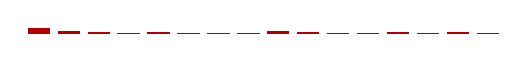
\begin{tikzpicture}[scale=0.38]
\foreach \i/\h in {0/0.22,1/0.10,2/0.08,3/0.05,4/0.07,5/0.04,6/0.04,7/0.03,
8/0.11,9/0.06,10/0.05,11/0.04,12/0.09,13/0.05,14/0.07,15/0.05}
	\fill[red!70!black] (\i,0) rectangle (\i+0.75,\h);
\end{tikzpicture}\\
\small Noisy $\mathbf{p}_{\mathrm{noisy}}$
\end{minipage}\hfill
\begin{minipage}{0.32\textwidth}
\centering
\begin{tikzpicture}[scale=0.38]
\foreach \i/\h in {0/0.32,1/0.085,2/0.065,3/0.035,4/0.055,5/0.025,6/0.025,7/0.015,
8/0.115,9/0.045,10/0.035,11/0.025,12/0.085,13/0.035,14/0.055,15/0.035}
	\fill[blue!60!black] (\i,0) rectangle (\i+0.75,\h);
\end{tikzpicture}\\
\small MLP $\hat{\mathbf{p}}$
\end{minipage}
\caption{نمایش مفهومی بازسازی توزیع: ایده‌آل (چپ)، نویزی (وسط)، خروجی \lr{MLP} (راست). هدف mitigation بازگرداندن شکل توزیع است، نه فقط بیشینه احتمال.}
\label{fig:dist-reconstruction}
\end{figure}

شکل~\ref{fig:dist-reconstruction} نشان می‌دهد چرا fidelity معیار مناسب‌تری از accuracy است: حتی اگر argmax یکسان بماند، توزیع کامل تغییر کرده و mitigation باید این تغییر را جبران کند.

\section{چالش‌ها، اصلاحات و نتایج}

\subsection{چالش‌های پروژه و راه‌حل‌ها}

پروژه فقط اجرای کد نبود؛ چند مشکل فنی در مسیر حل شد:

\begin{table}[htbp]
\centering
\caption{چالش‌های اصلی و اصلاحات انجام‌شده}
\label{tab:challenges}
\small
\begin{tabular}{p{3.2cm}p{5.2cm}p{4.8cm}}
\toprule
چالش & مشکل & راه‌حل \\
\midrule
ترتیب بیت‌ها & جابه‌جایی سطر/ستون $M$ & یکسان‌سازی \lr{bits\_to\_int} در همه بخش‌ها \\
قرارداد \lr{Qiskit} & transpose اشتباه ماتریس & $A_{ij}=P(m=j|p=i)$، اعمال $\mathbf{p}M$ \\
ماتریس $16\times16$ & \lr{Aer} کانال همبسته کامل ندارد & \lr{apply\_correlated\_readout\_noise} \\
\lr{ZZFeatureMap} یکنواخت & $F_{\mathrm{raw}}\approx0.972$، نویز کم‌اثر & افزایش \lr{reps} به ۲ \\
نویز train/test & ارزیابی cross-noise پیچیده & ارزیابی منطبق (matched) \\
\bottomrule
\end{tabular}
\end{table}

\subsection{بررسی چالش یکنواختی \lr{ZZFeatureMap}}

در فرآیند تولید داده برای ارزیابی عملکرد مدل یادگیری، یکی از چالش‌های مهم مربوط به استفاده از مدار
\lr{ZZFeatureMap}
مشاهده شد. در مراحل اولیه، داده‌های مربوط به این مدار با پارامترهای تصادفی و تعداد لایه کم
(\lr{reps=1})
تولید شدند. بررسی اولیه نشان داد که شباهت بین توزیع ایده‌آل و توزیع نویزی حتی پیش از اعمال مدل یادگیری بسیار زیاد است. به عنوان نمونه، مقدار فیدیلیتی خام بین داده‌های ایده‌آل و نویزی به صورت زیر مشاهده شد:

\begin{equation}
	F_{\mathrm{raw}} \approx 0.972
\end{equation}

این مقدار نشان می‌دهد که ورودی مدل (توزیع نویزی) و خروجی هدف (توزیع ایده‌آل) از ابتدا اختلاف بسیار کمی دارند. بنابراین اگر پس از آموزش مدل، مقدار فیدیلیتی بالایی مانند
$F \approx 0.996$
مشاهده شود، این نتیجه الزاماً نشان‌دهنده توانایی بالای مدل در یادگیری تصحیح نویز نیست، زیرا بخشی از این عملکرد ناشی از شباهت اولیه داده‌ها است.

بررسی توزیع‌های تولید شده نشان داد که دلیل اصلی این رفتار، ماهیت خروجی مدار
\lr{ZZFeatureMap}
با تنظیمات اولیه بود. این مدار در حالت
$\mathrm{reps}=1$
برای بسیاری از انتخاب‌های تصادفی پارامترها، توزیع احتمال حالت‌های اندازه‌گیری شده‌ای نزدیک به توزیع یکنواخت ایجاد می‌کند. در چنین شرایطی، اثر نویز خوانش روی توزیع احتمال کاهش پیدا می‌کند، زیرا تغییرات ایجاد شده توسط نویز در مقایسه با توزیع تقریباً یکنواخت بسیار کوچک است.

به بیان دیگر، مسئله اصلی در این مرحله، عدم صحت مدل نویز یا فرآیند اعمال ماتریس نویز نبود؛ بلکه داده‌های تولید شده از مدار، ساختار کافی برای آشکار کردن اثر نویز را نداشتند. در نتیجه مدل یادگیری ماشین عملاً با مسئله‌ای مواجه نبود که نیاز به اصلاح جدی داشته باشد.

برای رفع این مشکل، ساختار مدار تغییر داده شد و با افزایش عمق مدار از طریق افزایش تعداد لایه‌ها
($\mathrm{reps}=2$)
تنوع بیشتری در توزیع‌های خروجی ایجاد شد. هدف از این تغییر، ایجاد یک تعادل مناسب بین دو عامل بود:

\begin{itemize}
	\item وجود ساختار کافی در توزیع احتمال خروجی مدار، به طوری که مدل بتواند الگوهای کوانتومی را یاد بگیرد؛
	\item ایجاد اختلاف قابل مشاهده بین توزیع ایده‌آل و نویزی، به طوری که اثر نویز خوانش در داده‌ها باقی بماند.
\end{itemize}

پس از اصلاح مدار، مقدار خلوص توزیع‌های تولید شده افزایش یافت و در عین حال توزیع‌ها از حالت تقریباً یکنواخت خارج شدند. این تغییر باعث شد داده‌های تولید شده برای آموزش و ارزیابی مدل، چالش واقعی‌تری ایجاد کنند و عملکرد مدل در شرایط مختلف نویز قابل تفسیرتر باشد.

لازم به ذکر است که هدف در این پروژه، بیشینه کردن یا کمینه کردن مستقیم معیارهایی مانند
\lr{Purity}
یا
\lr{Fidelity}
نیست؛ بلکه هدف اصلی ایجاد دیتاست‌هایی است که در آن‌ها:
\begin{enumerate}
	\item مدارهای کوانتومی دارای ساختار قابل یادگیری باشند؛
	\item نویز خوانش بتواند تغییر قابل اندازه‌گیری در توزیع احتمال ایجاد کند؛
	\item مدل یادگیری مجبور به استخراج نگاشت بین توزیع نویزی و توزیع ایده‌آل باشد.
\end{enumerate}

بنابراین اصلاح پارامترهای مدار
\lr{ZZFeatureMap}
به عنوان یک مرحله ضروری در آماده‌سازی داده انجام شد تا ارزیابی مدل در مراحل بعدی پروژه، بازتاب واقعی‌تری از توانایی مدل در کاهش اثر نویز کوانتومی داشته باشد.
%===============


\subsection{جدول اصلی نتایج (ارزیابی با نویز منطبق)}

در ارزیابی نهایی، هر مدل آموزش‌دیده \emph{فقط} روی همان نویزی آزمون می‌شود که با آن آموزش دیده است؛ آزمون روی نویزهای نامرتبط انجام نمی‌شود. برای هر جفت $(\text{مدار}, \text{نویز})$، baseline از مدل هویت (بدون آموزش) و ستون \lr{Trained} از فاز متناظر به دست می‌آید. جدول~\ref{tab:main-fidelity} خلاصه میانگین fidelity روی ۱۵۰۰ نمونه test را نشان می‌دهد.

\begin{table}[htbp]
\centering
\caption{میانگین fidelity روی test با نویز منطبق train/test.}
\label{tab:main-fidelity}
\begin{tabular}{llccc}
\toprule
Circuit & Noise & Baseline & Trained & $\Delta F$\\
\midrule
\multirow{3}{*}{Independent}
& Synthetic & 0.907 & 0.979 & +0.072\\
& Exp.\ Single & 0.768 & 0.968 & +0.200\\
& Exp.\ Correlated & 0.763 & 0.984 & +0.221\\
\midrule
\multirow{3}{*}{ZZ FeatureMap}
& Synthetic & 0.938 & 0.973 & +0.035\\
& Exp.\ Single & 0.853 & 0.939 & +0.085\\
& Exp.\ Correlated & 0.861 & 0.974 & +0.113\\
\bottomrule
\end{tabular}
\end{table}

\subsection{تحلیل baseline}

ردیف \lr{Baseline} نشان می‌دهد نویز خوانش، پیش از mitigation، چقدر توزیع ایده‌آل را خراب می‌کند. برای مدار مستقل، fidelity نویز مصنوعی $0.907$ است، اما برای نویزهای تجربی به حدود $0.76$--$0.77$ افت می‌کند؛ یعنی نویز تجربی (تک‌کیوبیتی یا همبسته) حدود $14$--$15$ درصد همپوشانی بیشتری با ایده‌آل از بین می‌برد. برای \lr{ZZ FeatureMap} baselineها بالاترند ($0.85$--$0.94$)؛ شکل توزیع این مدار با همان نویزها در میانگین overlap بیشتری حفظ می‌کند، اما همچنان فضای قابل‌توجهی برای بهبود باقی می‌ماند.

\subsection{اثر آموزش با نویز منطبق}

وقتی train و test روی همان کانال نویز باشند، \lr{MLP} به‌طور پایدار fidelity را بالا می‌برد:
\begin{itemize}
	\item \lr{Independent/Synthetic}: $0.907 \rightarrow 0.979$ ($\Delta F = +0.072$)؛
	\item \lr{Independent/Exp.\ Single}: $0.768 \rightarrow 0.968$ ($\Delta F = +0.200$)؛
	\item \lr{Independent/Exp.\ Correlated}: $0.763 \rightarrow 0.984$ ($\Delta F = +0.221$)؛
	\item \lr{ZZ/Synthetic}: $0.938 \rightarrow 0.973$ ($\Delta F = +0.035$)؛
	\item \lr{ZZ/Exp.\ Single}: $0.853 \rightarrow 0.939$ ($\Delta F = +0.085$)؛
	\item \lr{ZZ/Exp.\ Correlated}: $0.861 \rightarrow 0.974$ ($\Delta F = +0.113$).
\end{itemize}
بیشترین بهبود مطلق در مدار مستقل و نویز همبسته رخ داده است ($\Delta F \approx 0.22$): جایی که baseline پایین‌تر بوده و مدل بیشترین فضا برای بازگرداندن توزیع داشته است. در \lr{ZZ FeatureMap}، چون baseline از ابتدا بالاتر است، $\Delta F$ کوچک‌تر است اما fidelity نهایی در هر سه نویز بالای $0.93$ باقی می‌ماند.

\subsection{نمودار fidelity: baseline در برابر آموزش}

شکل‌های~\ref{fig:fidelity-ind} و~\ref{fig:fidelity-zz} خروجی تابع \lr{plot\_fidelity\_bars} هستند و برای هر مدار، سه جفت میله (بدون آموزش / پس از آموزش منطبق) را نشان می‌دهند.

\begin{figure}[htbp]
\centering

\includegraphics[width=0.85\textwidth]{fidelity_ind.png}
\caption{مدار مستقل: مقایسه میانگین fidelity قبل و بعد از آموزش منطبق برای سه نوع نویز.}
\label{fig:fidelity-ind}
\end{figure}

برای مدار مستقل (شکل~\ref{fig:fidelity-ind})، میله‌های قرمز (baseline) در نویزهای تجربی به‌وضوح پایین‌تر از نویز مصنوعی‌اند. پس از آموزش، هر سه میله آبی به ناحیه $F > 0.96$ می‌رسند. بیشترین فاصله بین baseline و trained مربوط به \lr{Experimental Correlated} است ($\Delta F \approx 0.22$)؛ این نشان می‌دهد مدل حتی برای کانال نویز ۱۶$\times$۱۶ همبسته نیز نگاشت معکوس مؤثری یاد گرفته است.

\begin{figure}[htbp]
\centering

\includegraphics[width=0.85\textwidth]{fidelity_zz.png}
\caption{مدار \lr{ZZ FeatureMap}: مقایسه میانگین fidelity قبل و بعد از آموزش منطبق.}
\label{fig:fidelity-zz}
\end{figure}

در \lr{ZZ FeatureMap} (شکل~\ref{fig:fidelity-zz})، baseline نویز مصنوعی از ابتدا نزدیک $0.94$ است؛ بنابراین سود آموزش محدودتر ($\Delta F \approx 0.035$) ولی همچنان معنادار است. برای نویزهای تجربی، بهبود به ترتیب $+0.085$ و $+0.113$ است و fidelity نهایی به $0.97$ نزدیک می‌شود. این الگو با اصلاح \lr{reps} در مدار سازگار است: داده‌ها چالش کافی دارند و مدل همچنان قادر به mitigation است.

\subsection{داشبورد سه معیار}

شکل‌های~\ref{fig:metrics-ind} و~\ref{fig:metrics-zz} خروجی \lr{matched\_metrics\_dashboard} هستند و علاوه بر fidelity، \lr{L1} و \lr{KL} را در همان چارچوب matched گزارش می‌کنند.

\begin{figure}[htbp]
\centering

\includegraphics[width=\textwidth]{all_metrices_ind.png}
\caption{مدار مستقل: داشبورد سه معیار (fidelity، \lr{L1}، \lr{KL})؛ مقایسه بدون آموزش و پس از آموزش منطبق.}
\label{fig:metrics-ind}
\end{figure}

در مدار مستقل (شکل~\ref{fig:metrics-ind})، هر سه معیار یک داستان یکسان روایت می‌کنند: نویز تجربی baseline بدتری دارد (fidelity پایین، \lr{L1} و \lr{KL} بالا) و آموزش هر سه را به‌طور همزمان بهبود می‌دهد. برای \lr{Experimental Correlated}، \lr{L1} از حدود $0.72$ به $0.12$ و \lr{KL} از حدود $0.40$ به $0.02$ کاهش می‌یابد؛ یعنی شکل کامل توزیع ۱۶‌حالته بازسازی شده، نه فقط بیشینه احتمال.

\begin{figure}[htbp]
\centering

\includegraphics[width=\textwidth]{all_metrices_zz.png}
\caption{مدار \lr{ZZ FeatureMap}: داشبورد سه معیار در حالت ارزیابی منطبق.}
\label{fig:metrics-zz}
\end{figure}

در \lr{ZZ FeatureMap} (شکل~\ref{fig:metrics-zz})، الگوی مشابهی دیده می‌شود با دامنه متفاوت: baseline \lr{L1} برای نویزهای تجربی حدود $0.55$--$0.57$ است و پس از آموزش به $0.18$--$0.32$ می‌رسد. \lr{KL} نیز در همه حالت‌ها به زیر $0.12$ کاهش می‌یابد. نکته مهم این است که بهترین \lr{L1} و \lr{KL} نهایی مربوط به \lr{Experimental Correlated} است؛ در حالی که بیشترین $\Delta F$ در fidelity مربوط به همان نویز است---هم‌راستایی معیارها اعتبار نتایج را تقویت می‌کند.

\subsection{جمع‌بندی نتایج}

\begin{enumerate}
	\item \textbf{mitigation مؤثر است:} در هر شش سناریو، fidelity پس از آموزش از baseline بالاتر است و \lr{L1}/\lr{KL} کاهش می‌یابد.
	\item \textbf{نویز تجربی سخت‌تر است:} baseline پایین‌تر از نویز مصنوعی؛ بیشترین $\Delta F$ در مدار مستقل.
	\item \textbf{ارزیابی منطبق شفاف است:} هر سطر جدول~\ref{tab:main-fidelity} یک سوال مشخص را پاسخ می‌دهد: «آیا مدل آموزش‌دیده روی نویز $X$، توزیع را بهتر از مدل هویت بازمی‌گرداند؟»
	\item \textbf{مدار \lr{ZZ} baseline بالاتر، بهبود نسبی کمتر:} $\Delta F$ کوچک‌تر لزوماً ضعف نیست؛ fidelity نهایی همچنان بالای $0.93$ است.
\end{enumerate}

\section{محدودیت‌های فعلی پروژه}

\begin{enumerate}
	\item \textbf{مقیاس:} فقط ۴ کیوبیت بررسی شده؛ برای $n>4$ اندازه ماتریس $2^n\times2^n$ به‌سرعت رشد می‌کند.
	\item \textbf{وابستگی به کالیبراسیون:} ماتریس‌های نویز snapshot فعلی سخت‌افزار هستند و drift زمانی لحاظ نشده.
	\item \textbf{ارزیابی منطبق:} در این گزارش فقط حالت train/test matched بررسی شده؛ generalization به نویز یا مدار دیگر در scope فعلی نیست.
	\item \textbf{تقریب غیرخطی:} \lr{MLP} معکوس دقیق $M$ نیست؛ outside distribution ممکن است ضعیف عمل کند.
	\item \textbf{نویز فقط readout:} gate error و decoherence در شبیه‌سازی لحاظ نشده‌اند.
\end{enumerate}
بیان صریح این محدودیت‌ها اعتبار گزارش را بالا می‌برد و مسیر ادامه کار را روشن می‌کند.

\section{نکات حساس و توصیه‌های عملی}

\begin{enumerate}
	\item \textbf{ترتیب بیت‌ها}: قرارداد معادله~\eqref{eq:bits-to-int} باید در همه جا ثابت بماند. هر تغییر کوچک در ordering می‌تواند کل ماتریس $16\times16$ را جابه‌جا کند.
	\item \textbf{قرارداد سطری ماتریس}: همیشه $A_{ij}=P(m=j|p=i)$ است. بنابراین اعمال نویز همبسته به صورت $\mathbf{p}_{\mathrm{ideal}}M$ انجام می‌شود.
	\item \textbf{ماتریس $16\times16$ را با کرونکر اشتباه نگیریم}: کرونکر فقط مدل مستقل است؛ ماتریس تجربی کامل اطلاعات crosstalk و correlation را دارد.
	\item \textbf{نویز مصنوعی کافی نیست}: برای ارزیابی واقعی، باید حداقل از \lr{experimental\_single} و بهتر از آن از \lr{experimental\_correlated} استفاده شود.
	\item \textbf{مدل mitigation باید با شرایط آزمون سازگار باشد}: در این گزارش فقط ارزیابی منطبق انجام شده؛ train و test باید روی همان کانال نویز باشند.
\end{enumerate}

\section{جمع‌بندی نهایی}

این پروژه یک مسیر کامل و قابل دفاع برای مطالعه نویز خوانش چهار کیوبیتی ساخته است (شکل~\ref{fig:pipeline}). در بخش اول، داده‌های خام \lr{IQ} با \lr{LDA} به بیت‌های اندازه‌گیری‌شده تبدیل می‌شوند و پس از اعتبارسنجی، ماتریس‌های تخصیص تک‌کیوبیتی و ماتریس همبسته $16\times16$ استخراج می‌شود.

در بخش دوم، سه نوع نویز روی دو مدار کوانتومی اعمال می‌شود. ارزیابی نهایی \textbf{فقط} با نویز منطبق train/test انجام می‌شود؛ هر مدل روی همان کانالی آزمون می‌شود که با آن آموزش دیده است. مدل \lr{MLP} نقش تقریب کانال معکوس readout را دارد و با fidelity، \lr{KL} و \lr{L1} ارزیابی می‌شود (جدول~\ref{tab:main-fidelity} و شکل‌های~\ref{fig:fidelity-ind}--\ref{fig:metrics-zz}).

نتایج نشان می‌دهد mitigation در حالت منطبق بسیار مؤثر است: بیشترین بهبود fidelity ($\Delta F \approx 0.22$) برای مدار مستقل و نویز همبسته است؛ در \lr{ZZ FeatureMap} fidelity نهایی در هر سه نویز بالای $0.93$ باقی می‌ماند. برای کاربرد سخت‌افزاری، استفاده از ماتریس همبسته واقعی و آموزش/آزمون روی همان کانال نویز ضروری است.
